The current section present the work done on the stability analysis of the torque feedback. This is an ongoing work and here are presented preliminary results obtained as for now. Please keep in mind that all information contained here is subject to change.

In the current robot architecture, position $\theta$, commanded position  $\theta_d$ are sampled at 1~ms, while torque $\tau_f$ is refreshed approximately each 7~ms and command $u$ at 11~ms. These are the four main outputs usable for frequency response analysis, see fig.~\ref{fig:loop}. Therefore, data analysis has to be performed with these available data.

%\begin{figure}
%	\begin{center}
%		\def\svgwidth{173mm}%.75\textwidth
%		\input{./images/loop.pdf_tex}
%		\caption{Basic PI-D control loop with torque feedback}
%		\label{fig:loop}
%	\end{center}
%\end{figure}


%\subsection{Producing bode plots}\label{sec:bode}

%\subsection{Torque Loops}\label{sec:bode}
To trace a bode plot of the torque open loop, one needs the input $u$ and the output $\tau_c$, see fig.~\ref{fig:loop}. Output of the torque loop is computed from the output of the torque compensator:
\begin{align}
\tau_c &= K_{\tau}\tau_f. \label{eqn:tauc}
\end{align}

Previously, command $u$ was not considered usable for data analysis due to its slow refresh rate, i.e. 11~ms. The signal was thereby computed from position command $\theta_d$ and position feedback $\theta$. However, the command is logged before it is sent to the actuator. Difficulties in synchronizing in time the feedback information communicated by the actuator to the corresponding command led to a significant overestimation of the position error $\theta_{err}$ and therefore command $u$. In consequence, input of the torque open loop was overestimated and hence, the gain of the open loop was underestimated. The task of synchronizing these value was found not to be straight forward, justifying the use of the slowly refreshed command $u$.

As described in document "Kinova Actuator Controller", command sent to the motor is subject to clamping based on velocity and temperature. The measurement of the command is made after those limitation are applied. Therefore, if the clamping is considered part of the plant, since it is fixed by mechanical constraints and not subject to change, $u$ can be smaller than the actual output of the PID and the torque loop combined and can lead to an underestimation of the command sent by the controler. That could make an overestimation of the gain of the open loop and hence a underestimation of the gain and phase margin, i.e. worst margins than expected. However, in the frequency responses performed for the current analysis, command $u$ mostly remained under the limitation imposed, especially in the frequency range were the stability margins are observed.


\subsection{Test Method}

\begin{itemize}
	\item Sine-swept
	
	Due to the current firmware limitations, frequency responses can be performed using position inputs only. It is known that this is not ideal to perform stability analysis of the torque loop. Moreover, having the position loop active affect the results.
	
	The sine-swept is sent accordingly to the following equation: ??
	
	Tested range of frequency is from 0 to 38Hz. To prevent damage to the robot, for each configuration, a first test covering the whole range of frequency is performed with a small half-amplitude of 0.05~deg. In a second test, the half-amplitude is raised to 0.1~deg and the frequency range is limited to where margins are observed.
	
	\item Test setup
	
	To perform frequency responses, the robot is attached to an aluminum bed with a steel plate of 1/2 inch. Therefore, flexibility of the bed, the steel plate and even the movement of the bed relative to the ground affect results. A picture of the test setup is shown in fig.~\ref{fig:bed}.
	
	\item End effector mass
	
	Assuming that the arm is used in operation with an IDM, a mass is attached to the robot for all frequency responses performed to obtain the data presented in the current document. The mass of the end effector is 1.3~kg.
	
	\item Configuration tested
	
	To perform a broad analysis, yet without performing an unnecessary large number of tests, a set of configurations covering a range over joint 2 and joint 4 is used. These joints are known to be affecting inertia the most. Moreover, a set of clinical arm configurations have been sent previously to Kinova for maximum insertion and retraction force. Since they represent normal operation configurations, they have been tested too. However, the joint 1 angle has been modified for each configuration to keep the arm above the test bed. The basic configuration and the 10 clinical cases are presented in table~\ref{table:cases}.

	

\end{itemize}

	\begin{table}[t]
		\centering
		\caption{Stability analysis: tested configurations}
		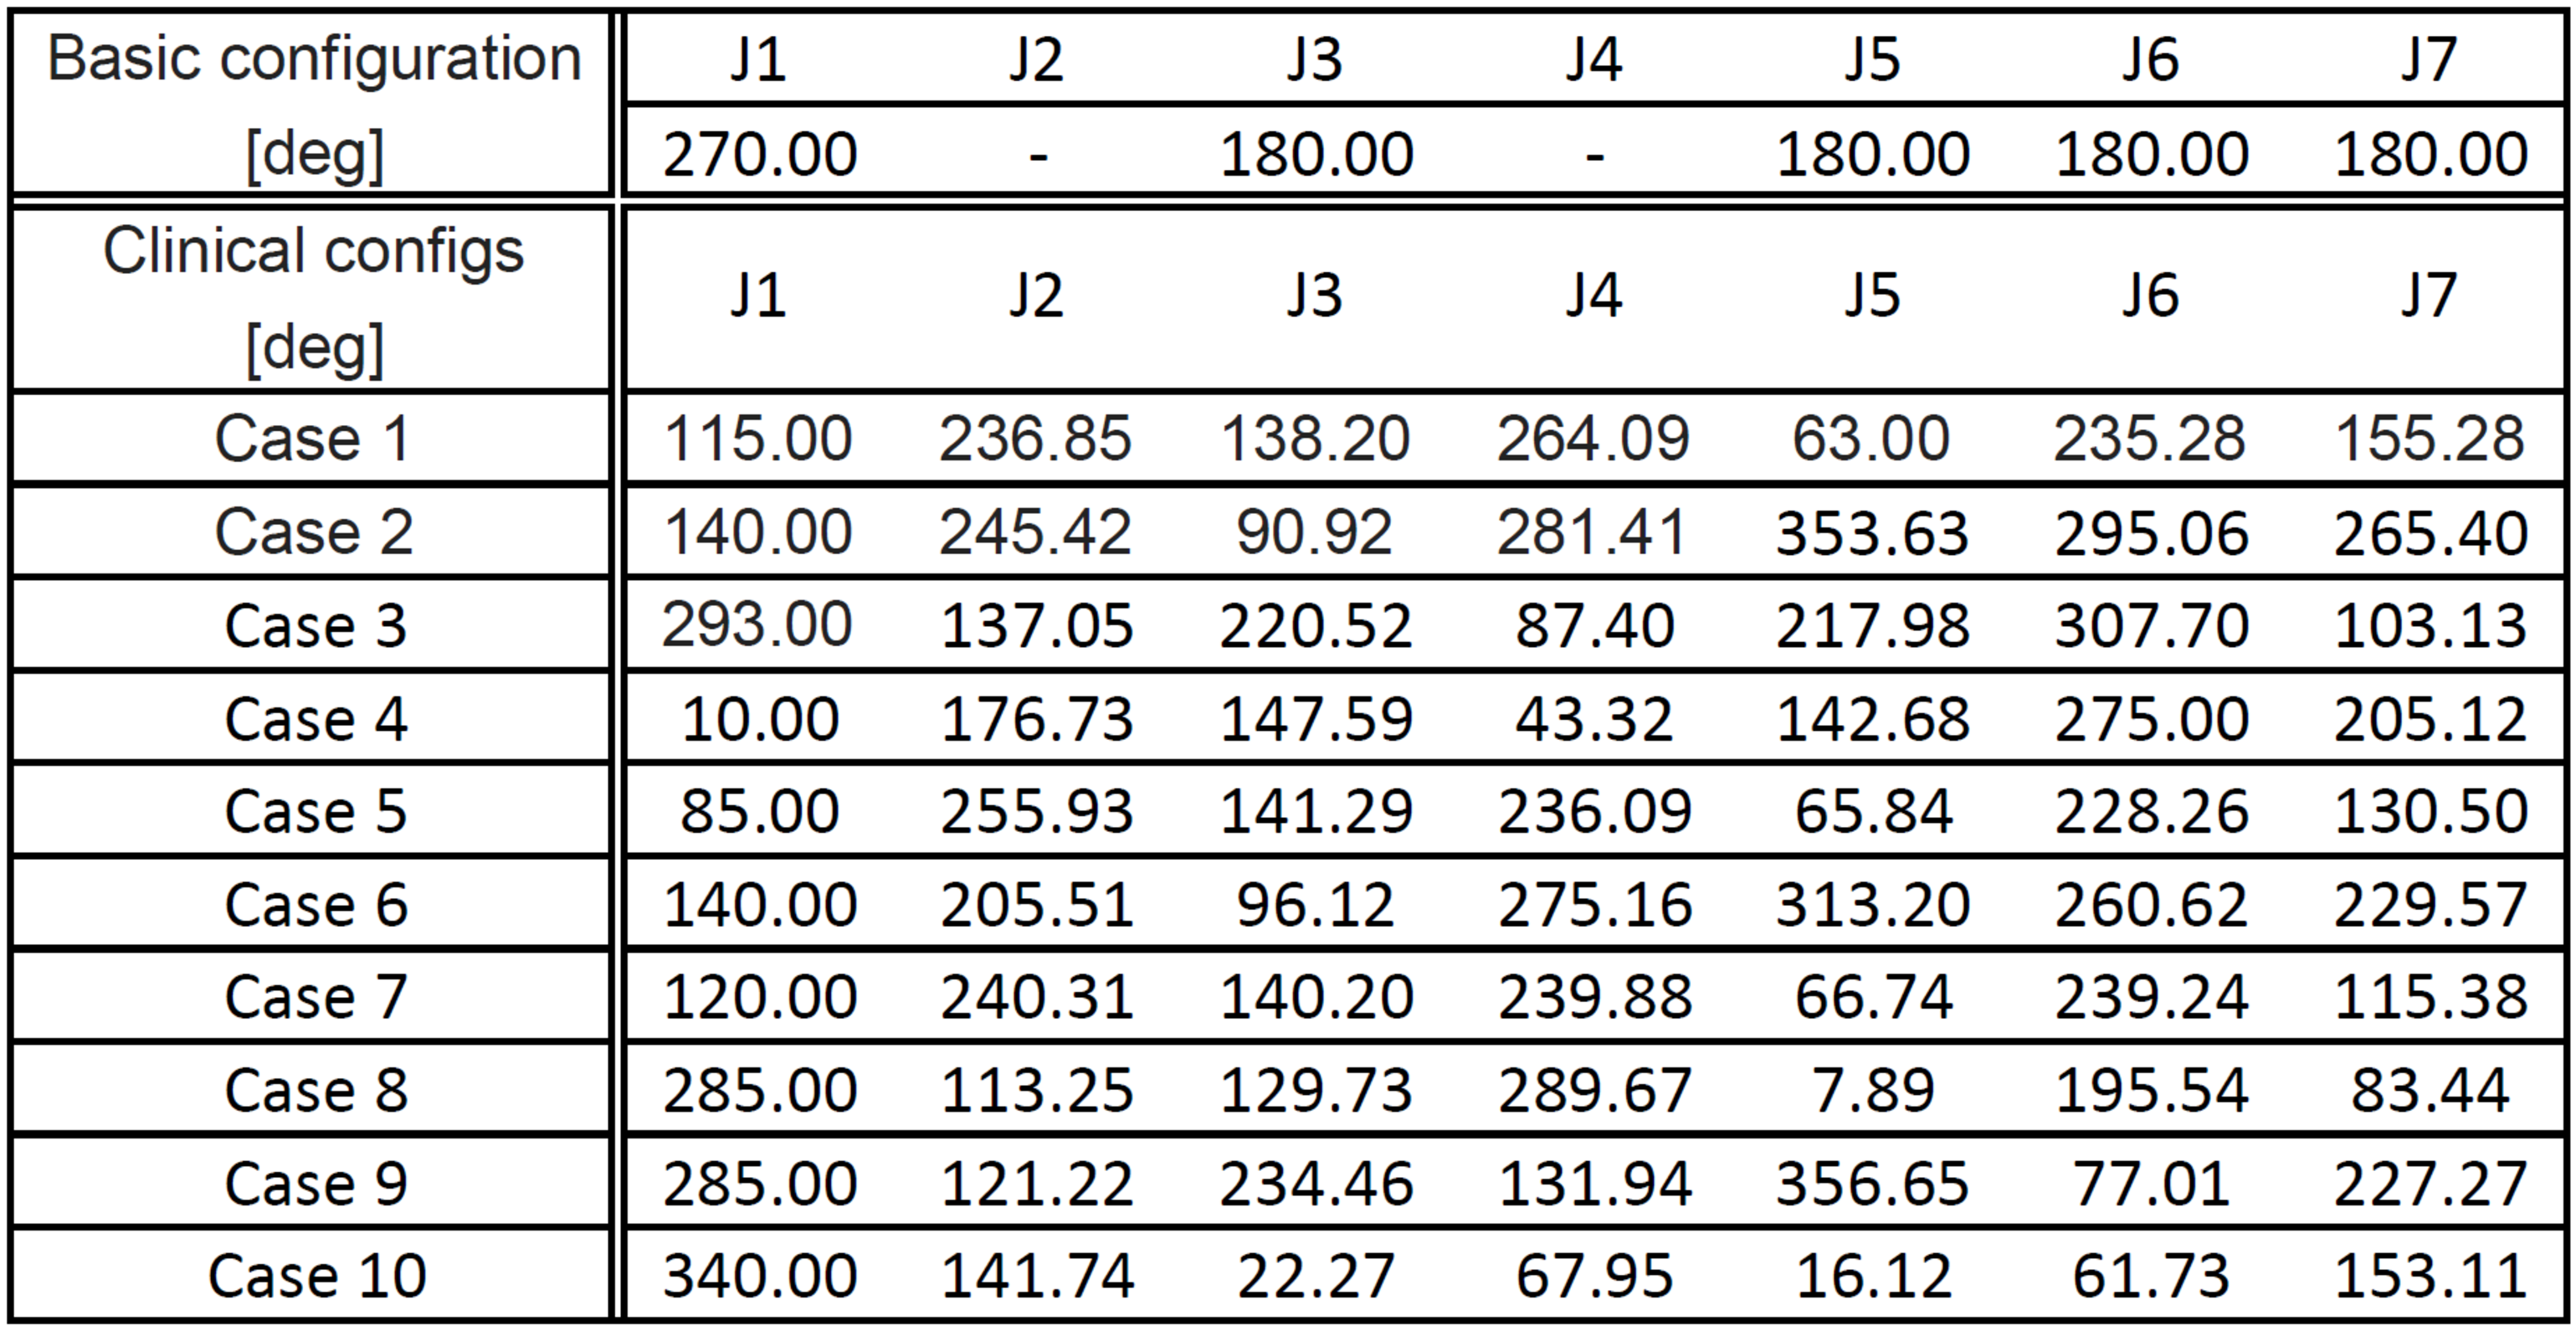
\includegraphics[width=.8\textwidth]{./images/configs.pdf}%
		%		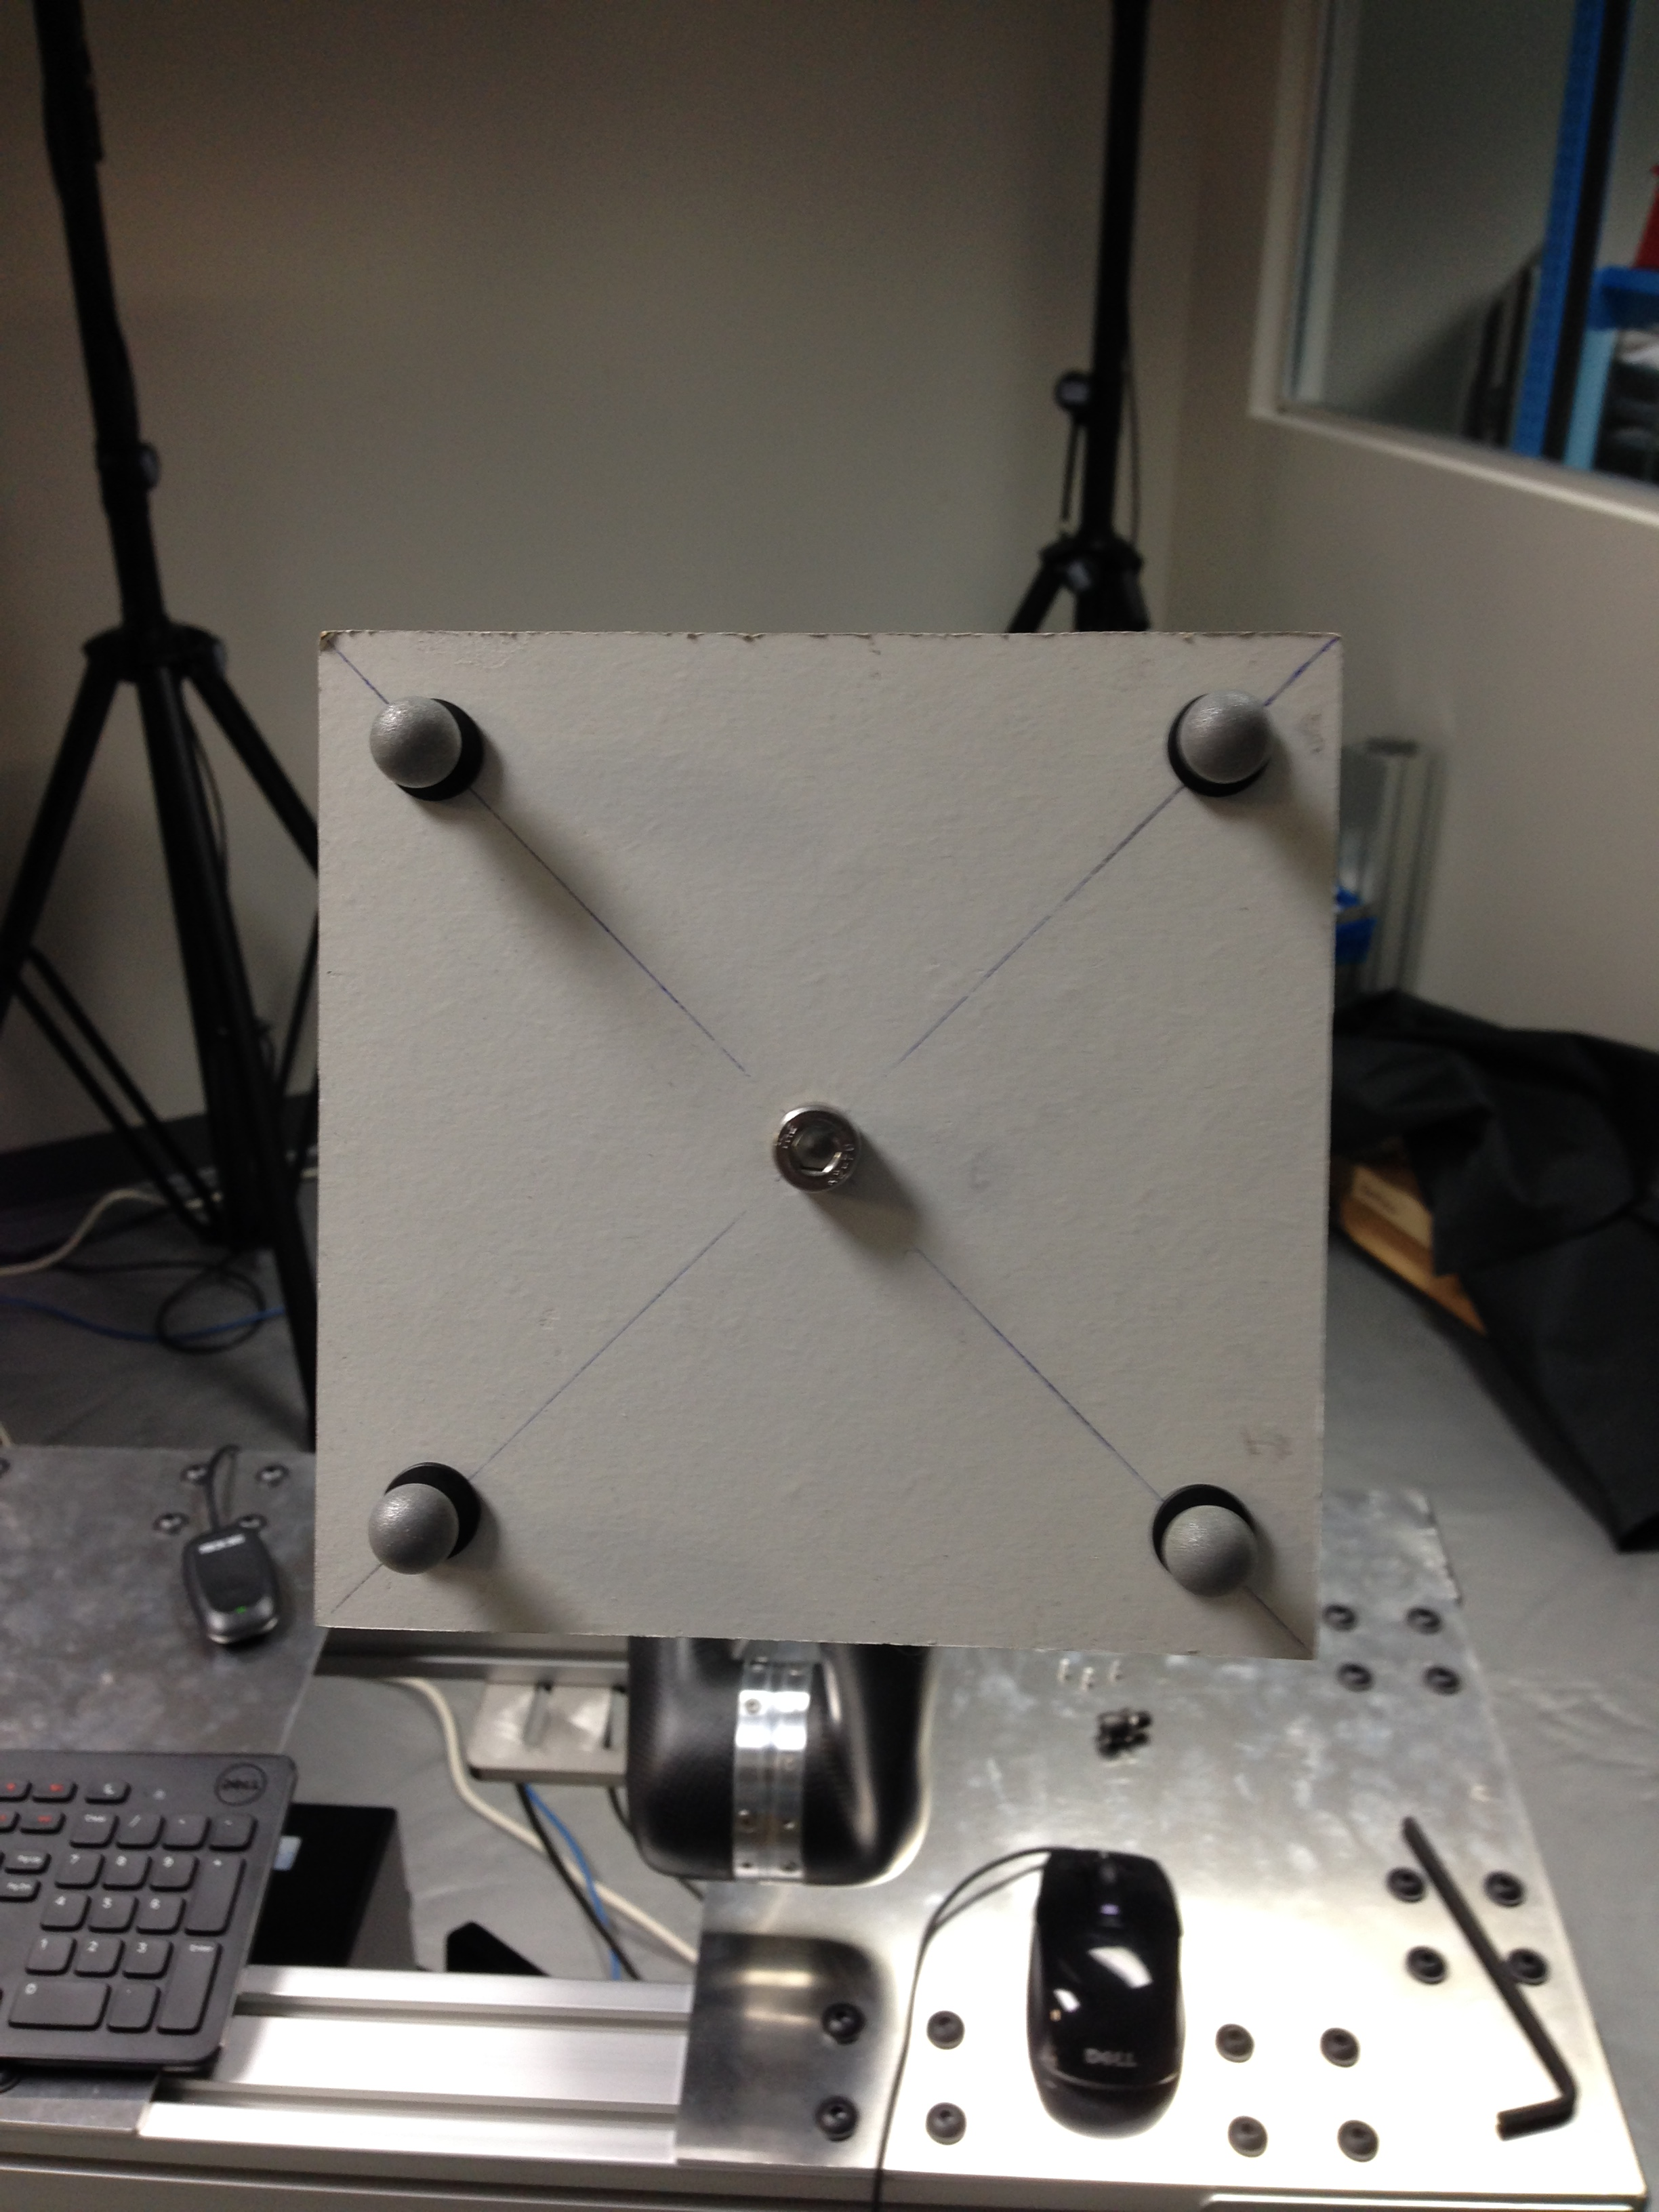
\includegraphics[width=0.5\textwidth]{./images/test_setup_2.JPG}%
		% test_setup
		\label{table:cases}
	\end{table}

\begin{figure}
	\begin{center}
		%\begin{table}[t]
		%	\centering
		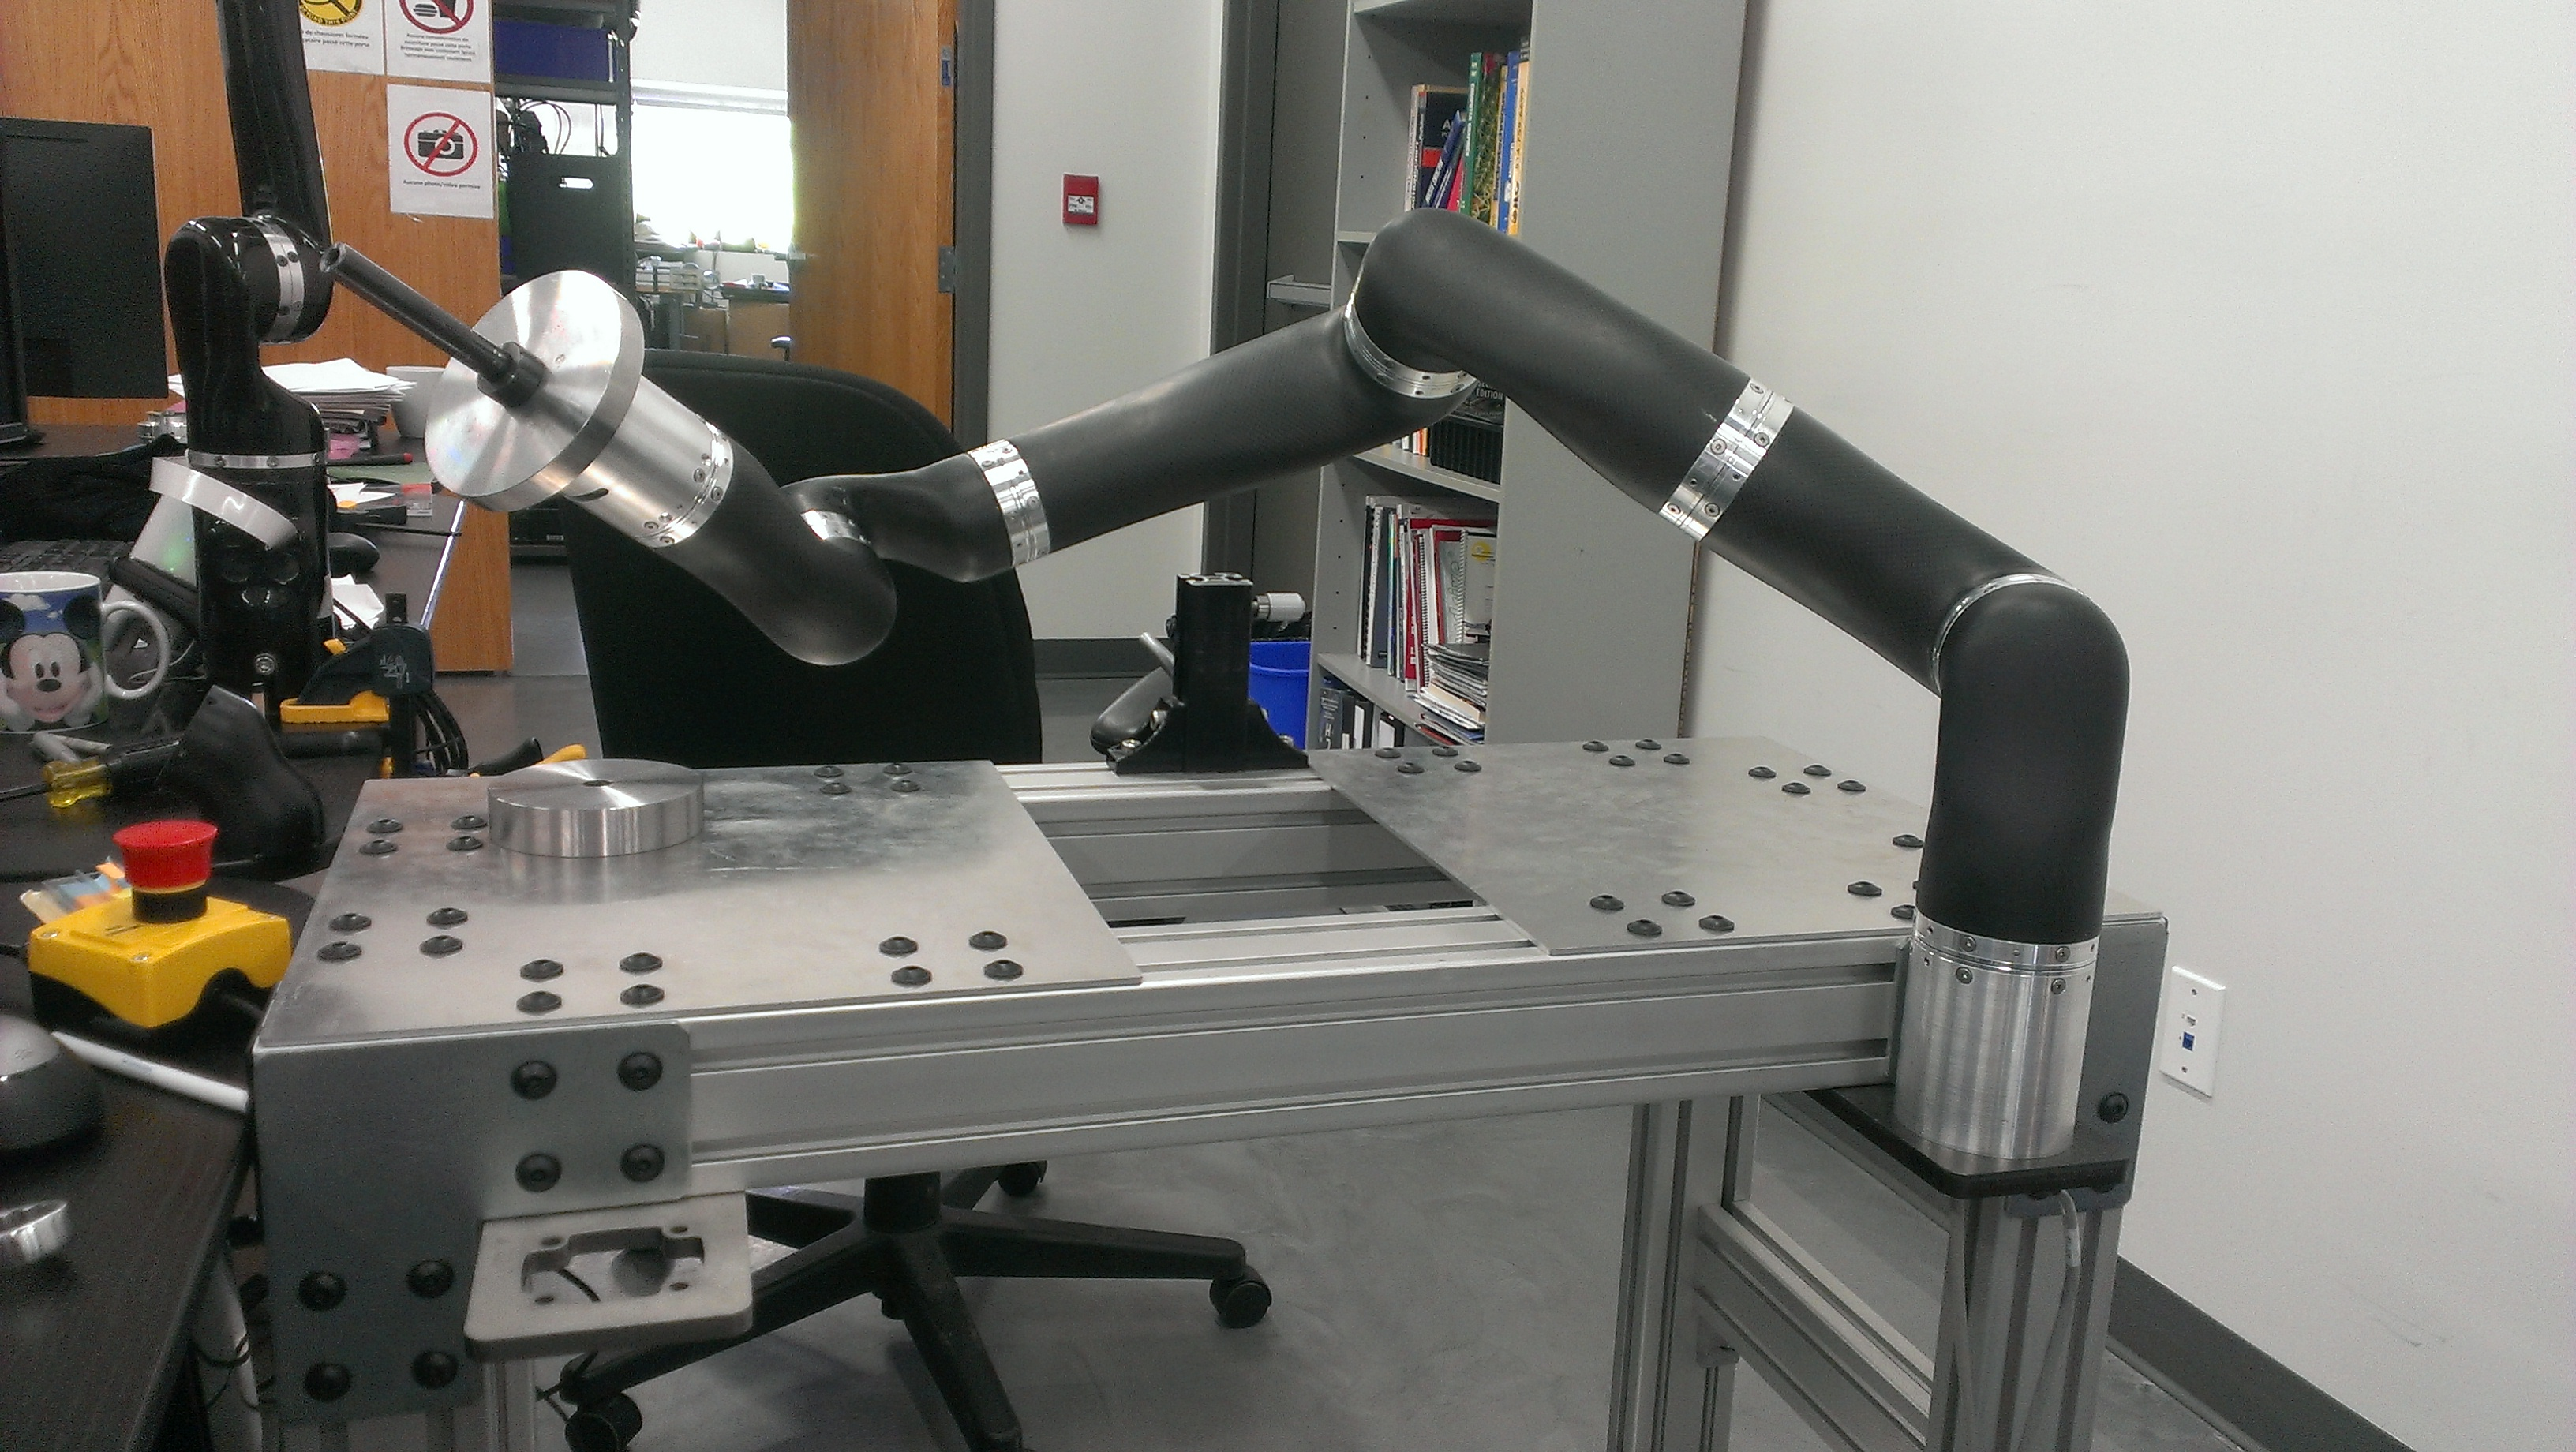
\includegraphics[width=1\textwidth]{./images/bed.jpg}%
		\caption{Test setup for frequency responses}
		\label{fig:bed}
		%\end{table}
	\end{center}
\end{figure}


%The robot end effector is moved back and forth between two points along a diagonal in the robot workspace, see fig.~\ref{fig:path}. The trajectory is from XYZ (0.5,-0.5,0.45) to (0.25,0.6,-0.1) in meters and is repeated 9 times. Optitrack camera system is used to track the end effector. The test is performed at 30 mm/s and 50 mm/s on two different robots. Tests at 50 mm/s (above maximal nominal speed) show more vibration and better demonstrate the vibration damping from torque feedback.

\begin{figure}
	\begin{center}
	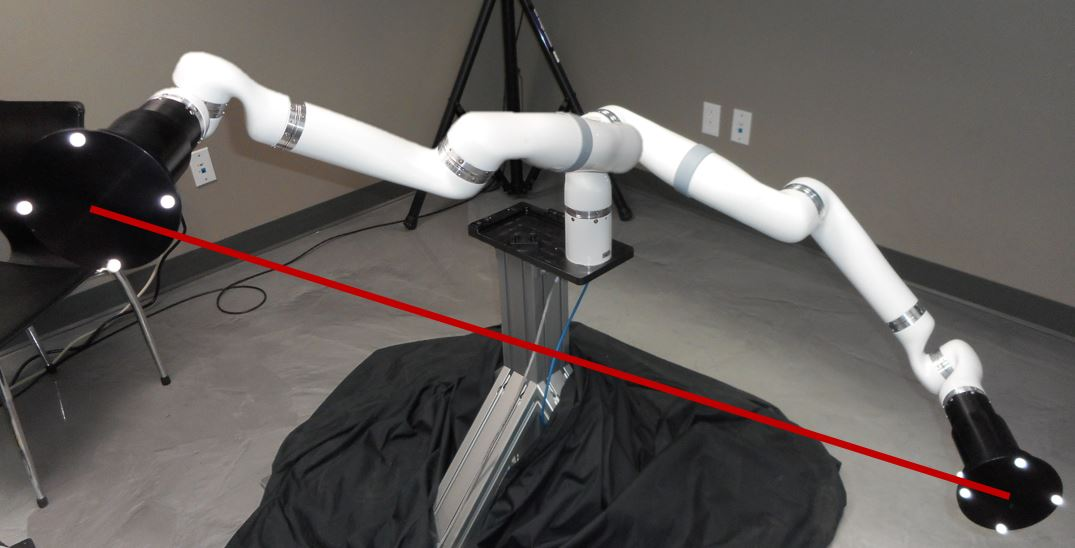
\includegraphics[width=.8\textwidth]{./images/testPath.jpg}%
		\caption{Test Trajectory}
	\label{fig:path}
	\end{center}
\end{figure}

From previous tests, vibration frequencies are known to be above 5~Hz. Therefore, a high-pass filter at 1~Hz is applied on the collected data to isolate vibration.  The mean, standard and maximum deviations are computed from it. Filtered data from two parts (over the 9) of the trajectory are shown in fig.~\ref{fig:data}. Regions of the trajectory showing worst behavior in terms of vibration are isolated and the same (but local) analysis is performed, see enclosed regions in fig.~\ref{fig:data}. All results are shown in table~\ref{table:results_torque}.

\begin{figure}
	\begin{center}
			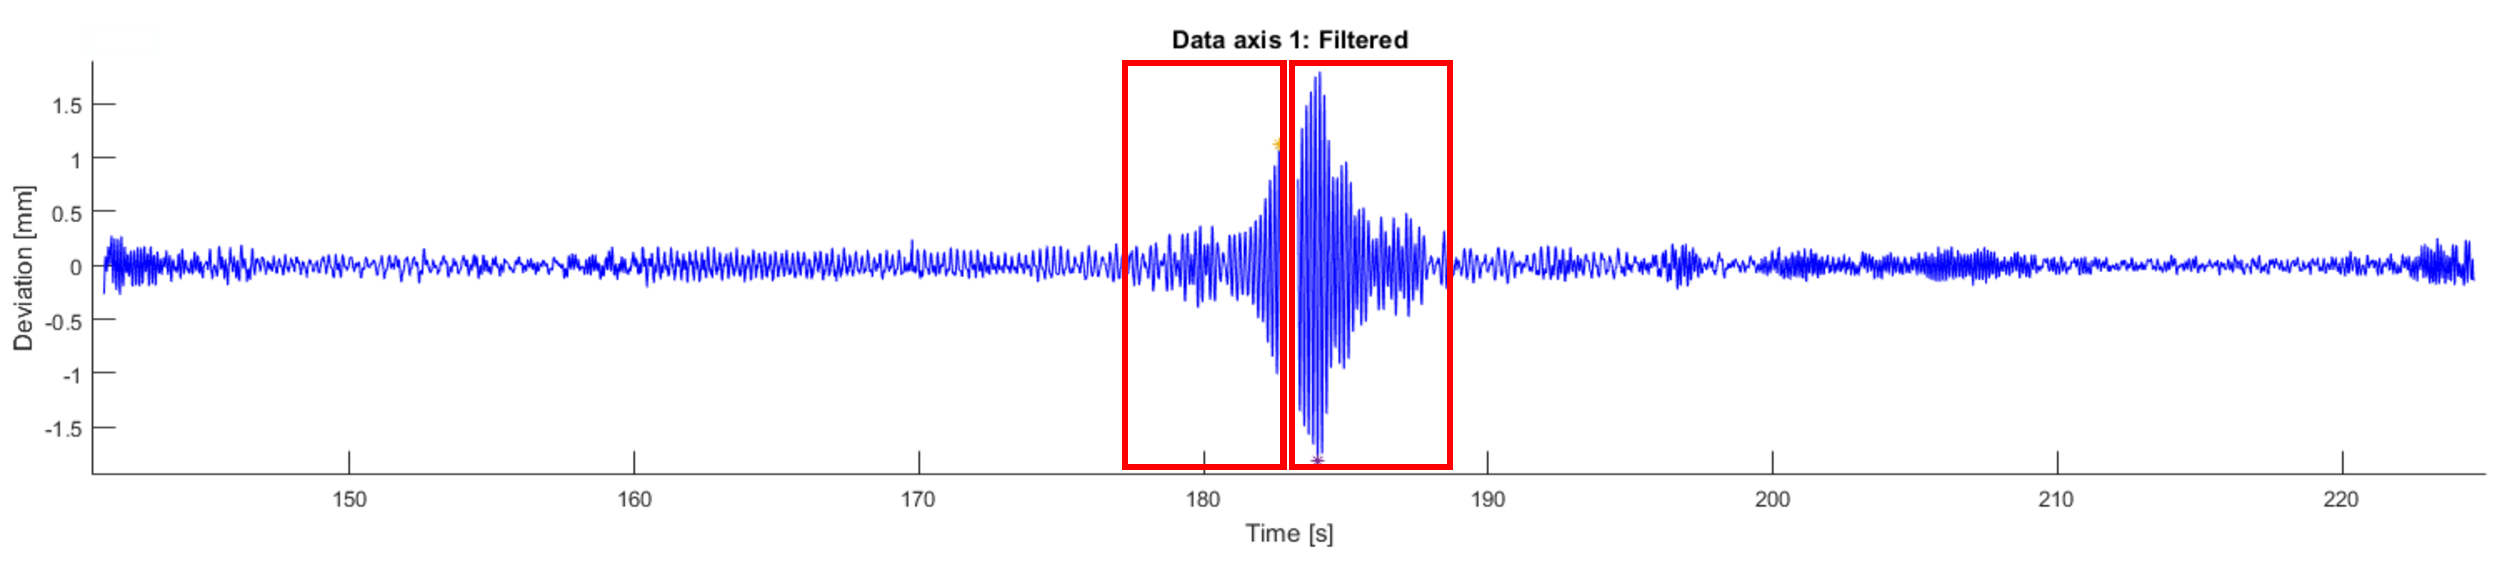
\includegraphics[width=1\textwidth]{./images/data2.pdf}%
			\caption{Filtered data from 2 parts of the trajectory and selected region for local analysis - Errata mm should be m}
			\label{fig:data}
	\end{center}
\end{figure}


\subsection{Data Analysis}
\begin{itemize}
	\item Matlab ??
\end{itemize}

\subsection{Preliminary Results}

Margins computed from the frequency responses are shown in table~\ref{table:SAtable}. According to those results, torque open loop is mainly unstable or close to instability. However, no instability is observed in operation. The whole controller is therefore most likely to be stable, i.e. position and torque closed loop running at the same time. However, open loops should show acceptable stability margins. Unfortunately, actual torque feedback parameters were set before the completion of the current analysis and previous frequency responses analysis were underestimating the gain.

Since most margins are observed around the same frequencies, namely around 13~Hz, more than simply reducing gains, i.e. modification of the torque compensator, reducing phase lag at that frequency for example, could help in stabilizing the torque loop. Open loop gain can also vary significantly between two configurations. Gain scheduling could therefore offer better performance and stability.

Typical bode plots of the torque open loop are shown in fig.??. One can notice that the frequency response can vary significantly from one configuration to the other and for one actuator to the other. Torque loops could benefit from different compensators for each joint and even for different configurations.


	\begin{table}[t]
		\centering
		\caption{Stability analysis results: gain margins, phase margins and corresponding frequencies}
		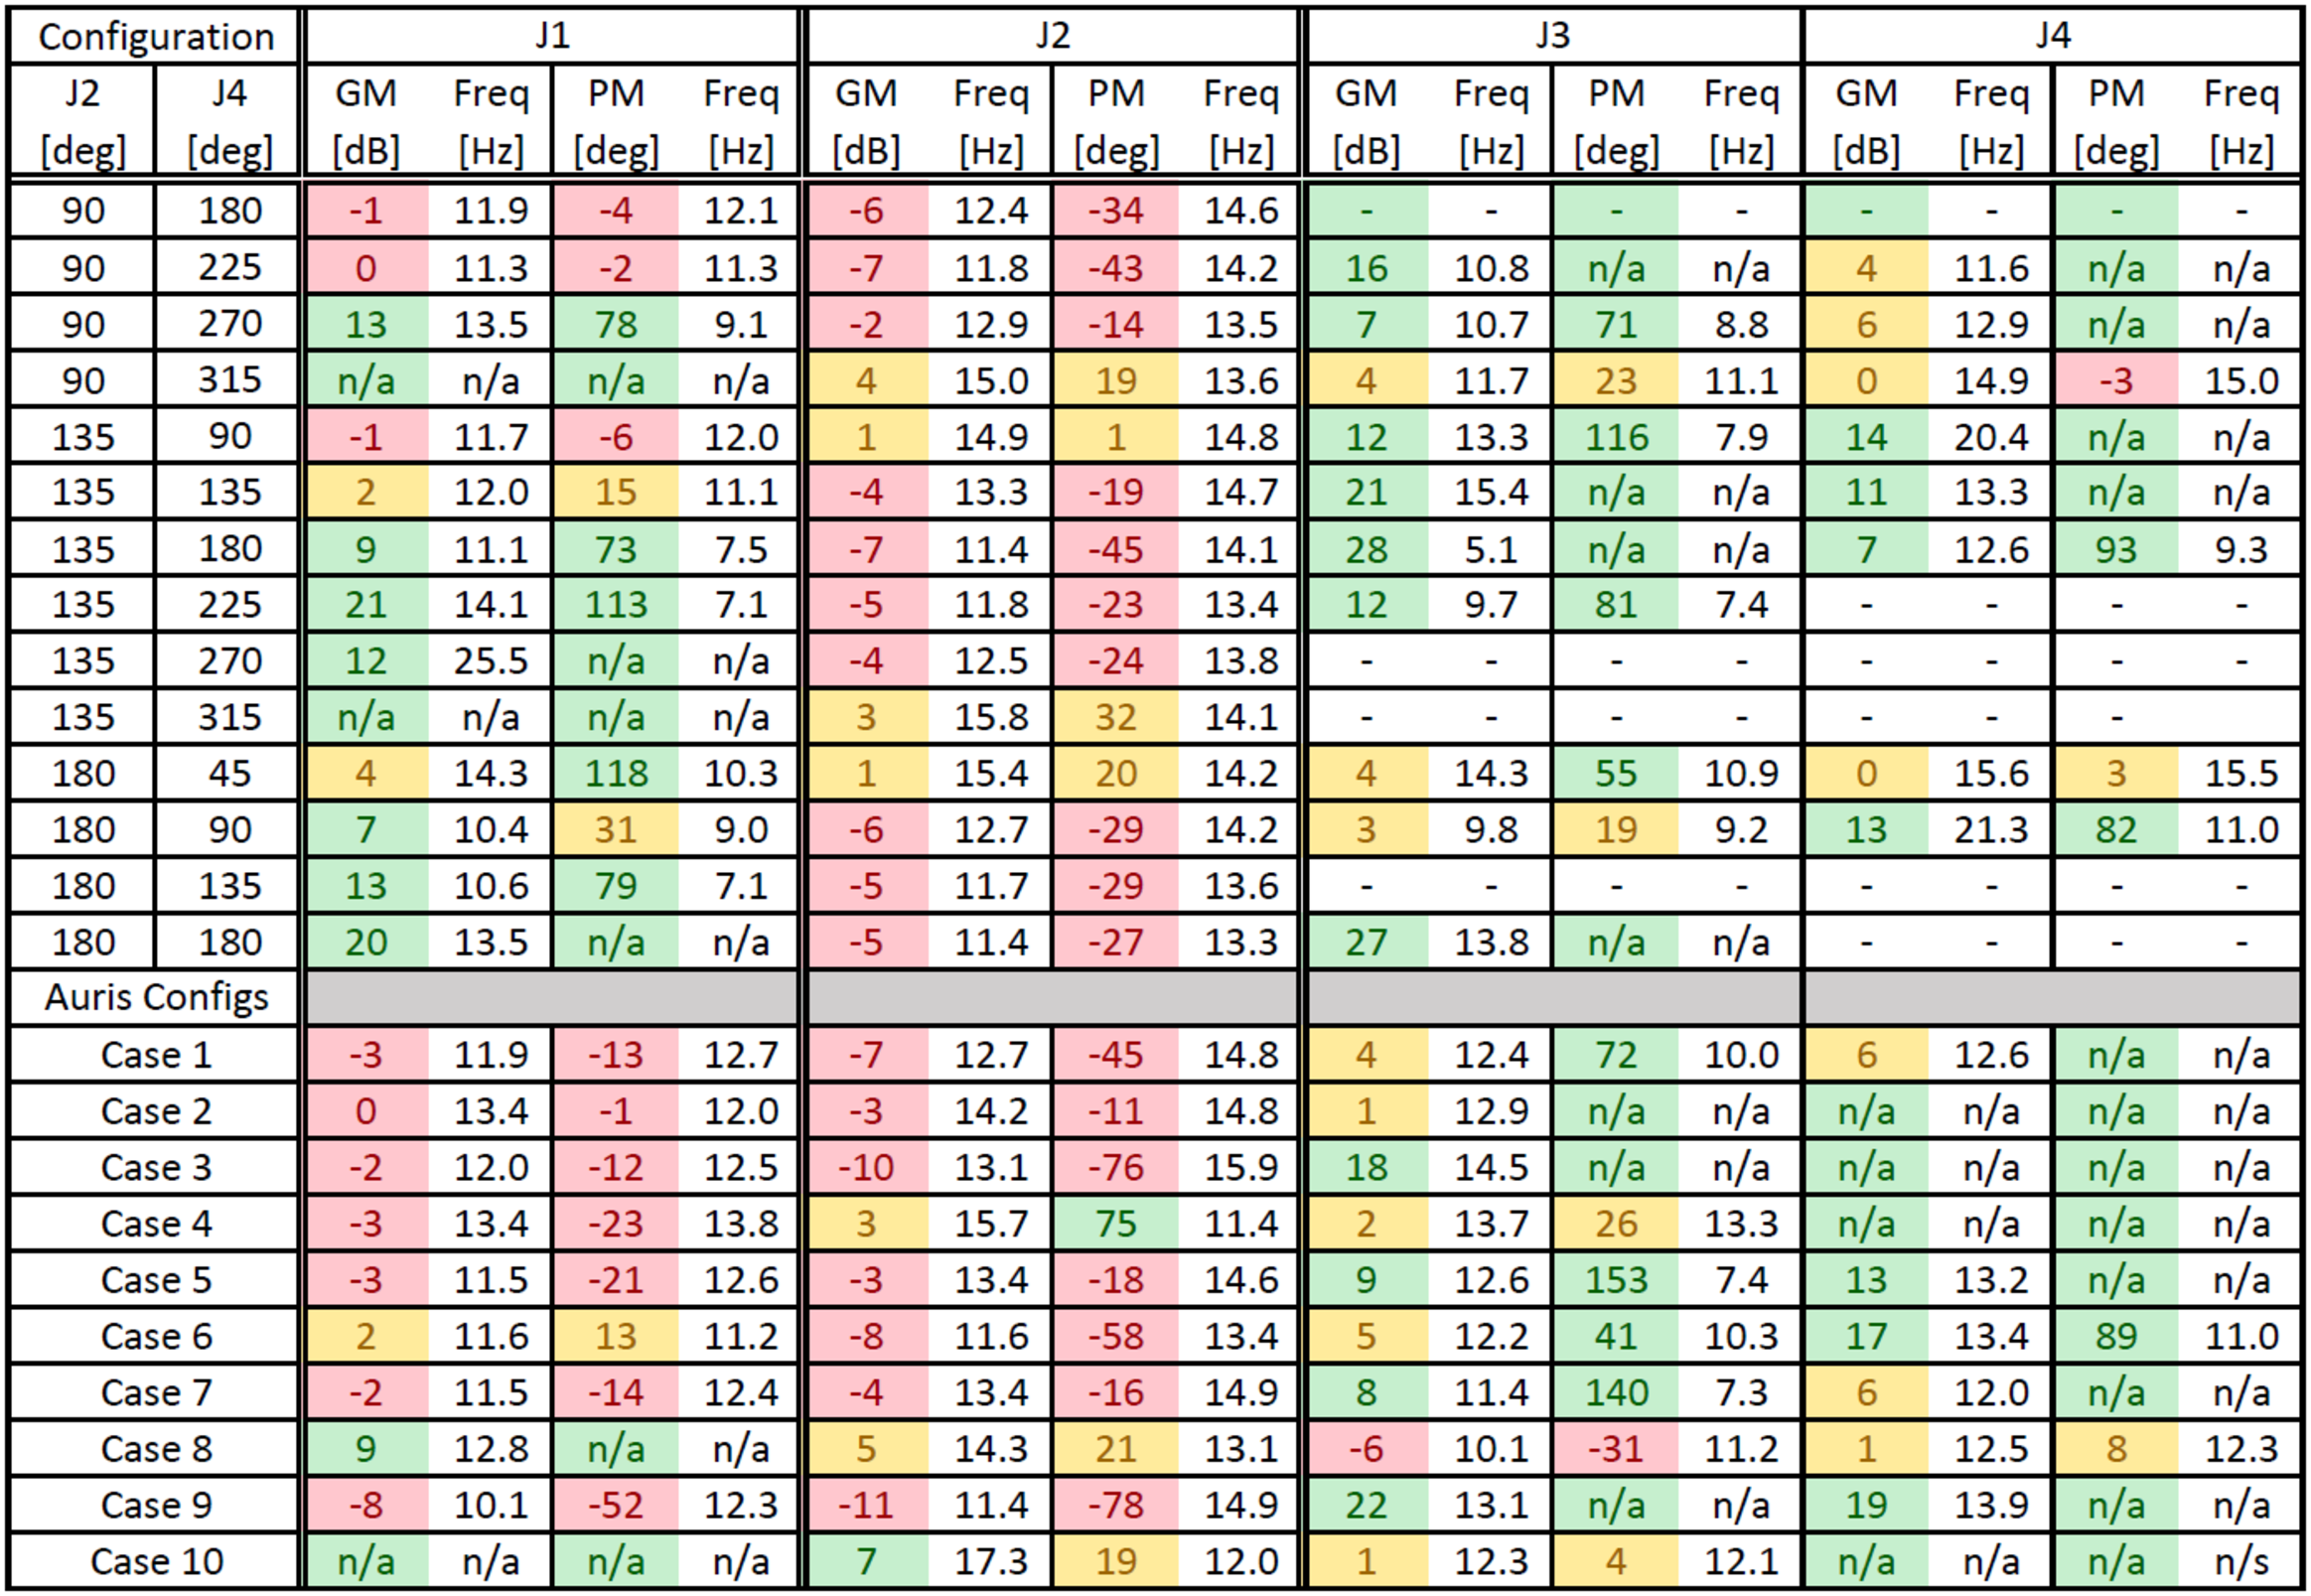
\includegraphics[width=1\textwidth]{./images/SAtable.pdf}%
		%		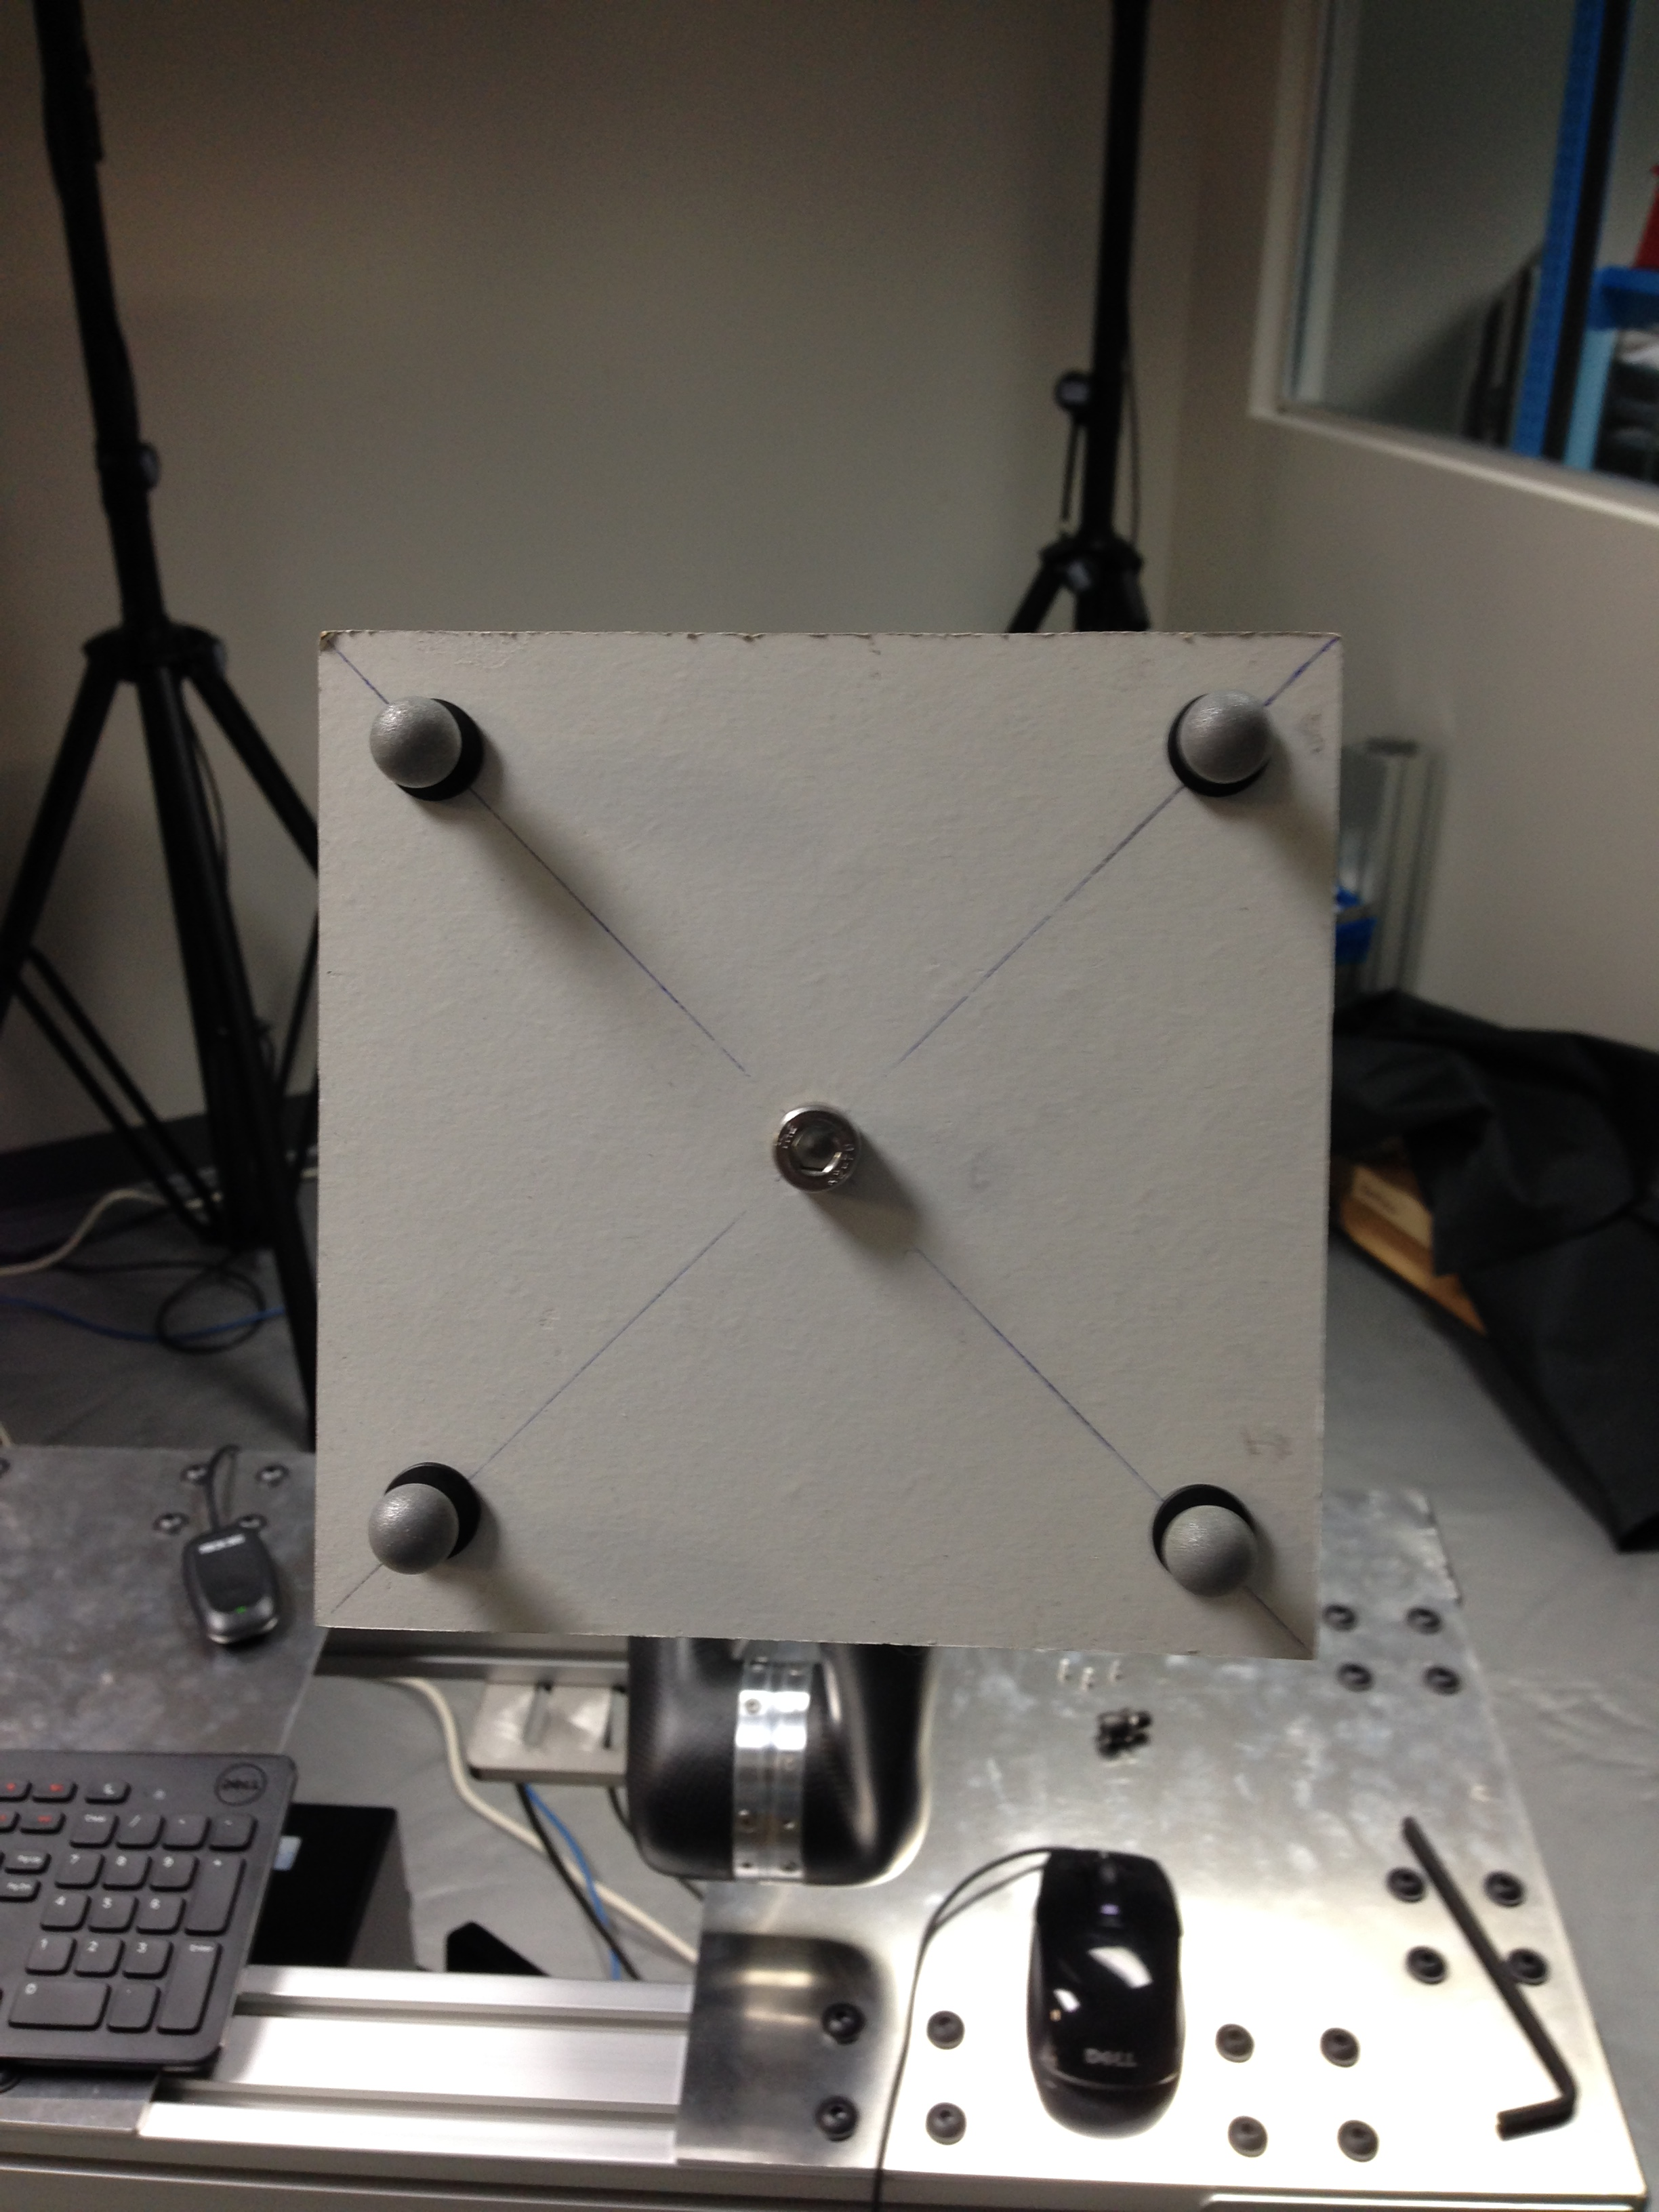
\includegraphics[width=0.5\textwidth]{./images/test_setup_2.JPG}%
		% test_setup
		\label{table:SAtable}
	\end{table}


\subsection{Concerns about current method and results}
\begin{itemize}
	\item Datalog
	
	Slow refresh rates and difficulty to synchronize data represent a important factor of error. Getting better refresh rate, more data outputs and a deeper analysis to synchronize data would greatly enhance confidence in the data collected and results obtained. 
	
	\item Sine-swept in position
	
	The limitation to the use of a sine-swept in position does not allows the deactivation of that particular loop. The position loop is therefore affecting the behavior of the system and reduce confidence in the results obtained for the torque loop. The capacity to activate and deactivate both loop separately and dive torque inputs to the corresponding loop would be a significant enhancement. 
    
    \item Data validation
    
    Very little data validation has been not yet. This is an important process to ensure collected data and results represent the behavior of the system.
    
	\item Analysis tools
	
	Further study of the analysis tools, mainly MATLAB data analysis functions, would be preferable to validate results.
	
\end{itemize}